Tato kapitola rozebírá, k~čemu slouží zaznamenávání odpracovaného času. Poté popisuje možnosti, které umožňují měření času spouštět a také se věnuje příkladům řešení, která již pro zaznamenávání odpracovaného času existují. V dalších sekcích se poté obecně zaměřuje na vývoj aplikací pro mobilní platformu iOS včetně možností multiplatformního a cross-platformního vývoje. Na závěr poté zkoumá, jaké existují možnosti pro integraci spouštěčů měření odpracovaného času a exportu dat do dalších aplikací.

%---------------------------------------------------------------
\section{Zaznamenávání odpracovaného času}
%---------------------------------------------------------------

Zaznamenávání odpracovaného času může být potřeba z~několika různých důvodů, buď z~pohledu jednotlivce, nebo z~pohledu spolupráce v~nějakém týmu. Mezi tyto důvody může patřit například:
\begin{itemize}
\item\textbf{Sledování pracovních hodin:} Pomáhá zaměstnancům a podnikům sledovat, kolik času strávili na různých úkolech, projektů a aktivitách během pracovní doby. To může být užitečné pro sledování produktivity, hodnocení efektivity práce a plánování rozpočtu času.
\item\textbf{Fakturace a účtování:} Pro profesionály a firmy, které účtují za své služby na základě odpracovaného času, umožňuje zaznamenávání snadné sledování času stráveného na jednotlivých projektech a klientech pro účely fakturace.
\item\textbf{Analýza produktivity:} Poskytuje data a statistiky o~tom, jaký čas je věnován různým úkolům a projektům. To umožňuje identifikovat trendy v~pracovních návycích, optimalizovat časové plánování a zlepšit efektivitu práce.
\item\textbf{Správa projektů:} Pomáhá organizovat časové údaje spojené s~různými projekty a úkoly, což usnadňuje plánování, delegování a monitorování pokroku.
\item\textbf{Transparentnost a komunikace:} Pro týmy umožňuje transparentně sdílet informace o~čase stráveném na různých aktivitách, což podporuje spolupráci a komunikaci v rámci týmu.
\end{itemize}

Celkově zaznamenávání slouží k~lepšímu řízení času, sledování produktivity a optimalizaci využití pracovního času pro jednotlivce i~organizace.

\begin{figure}[h]
	\centering
	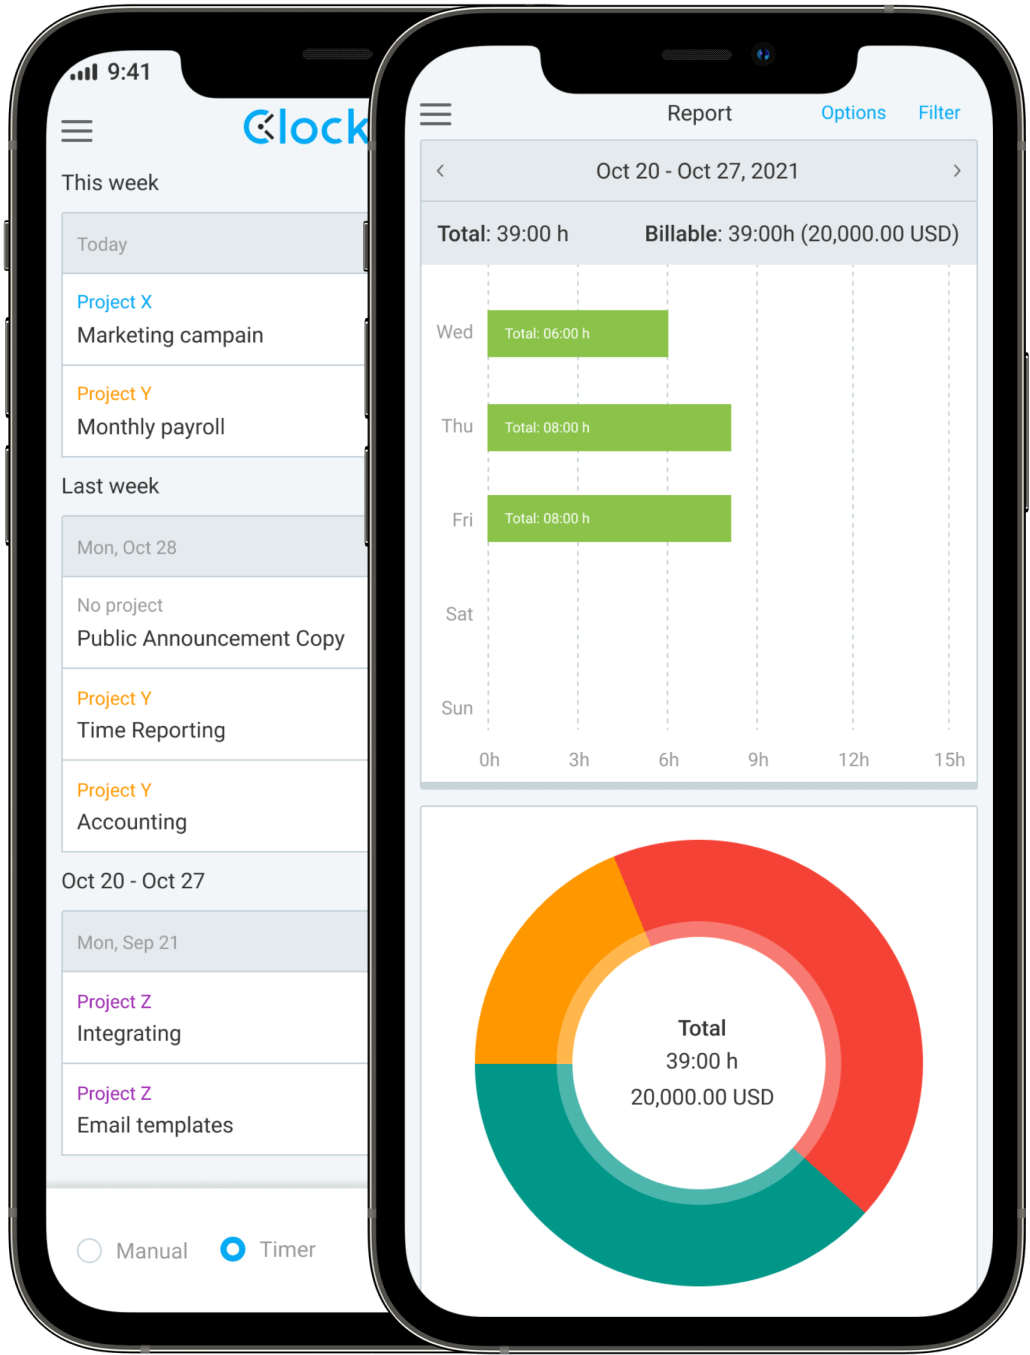
\includegraphics[width=10cm]{clockify-ios.png}
	\caption{Clockify – iOS aplikace pro měření času \cite{clockify-ios}}
	\label{fig:clockify-ios}
\end{figure}

%---------------------------------------------------------------
\section{Spouštěče měření času}
%---------------------------------------------------------------

Jedním z~cílů této práce je prozkoumat různá řešení pro spouštěče měření času. Nejjednodušším spouštěčem je samozřejmě ruční zapnutí nějaké formy časovače v~samotné aplikaci, která pro měření času slouží. To ale umí kdejaké již existující řešení a přidanou hodnotou této práce by měly být nějaké možnosti, jak spouštění uživateli ulehčit. Tyto možnosti se dají rozdělit do dvou kategorií – fyzické a softwarové.

%---------------------------------------------------------------
\subsection{Fyzické}
%---------------------------------------------------------------

Za fyzické spouštěče měření času lze považovat jakoukoli formu fyzického ovladače, kterou může uživatel nějak ovládat a tím spouštět časovač měření času.

Častým typem fyzického spouštěče je nějaká forma takzvaného platónského tělesa (krychle, osmistěn, dvanáctistěn, atd.), které může uživatel otáčet. Podle toho, na kterou stranu ho položí, tak se spustí časovač s danými parametry. Různé strany tělesa mohou sloužit například pro identifikování toho, na kterém projektu uživatel zrovna pracuje.

Mezi fyzické spouštěče patří například tyto produkty:
\begin{itemize}
\item\textbf{TIMEFLIP:} Dvanáctistěnné těleso, na které si uživatel může nalepovat cokoli, co bude identifikovat odpracovaný čas. Těleso se propojí s~mobilní aplikací, která poté spravuje naměřený čas. \cite{timeflip}
\item\textbf{TIMEULAR:} Stejný princip jako \emph{TIMEFLIP}, akorát používá osmistěnné těleso. Jednotlivé strany jdou také přizpůsobovat nálepkami. \cite{timeular}
\item\textbf{timeBuzzer:} Fyzické tlačítko, které lze umístit na stůl a zapojit do počítače. Stisknutí tlačítka otevře okno měřící aplikace, otočením tlačítka lze vybrat projekt a opětovným stisknutím se začne daný projekt měřit. \cite{timebuzzer}
\end{itemize}

\begin{figure}[h]
	\centering
	\begin{subfigure}[b]{5.2cm}
		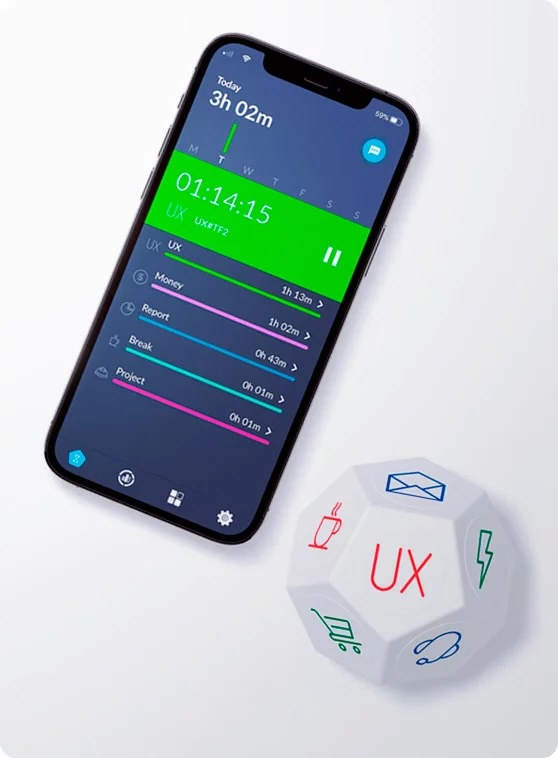
\includegraphics[width=5.2cm]{timeflip.jpeg}
		\caption{TIMEFLIP – Kostka a aplikace \cite{timeflip}}
		\label{pic:timeflip}
	\end{subfigure}
	\hspace{2cm}
	\begin{subfigure}[b]{7cm}
		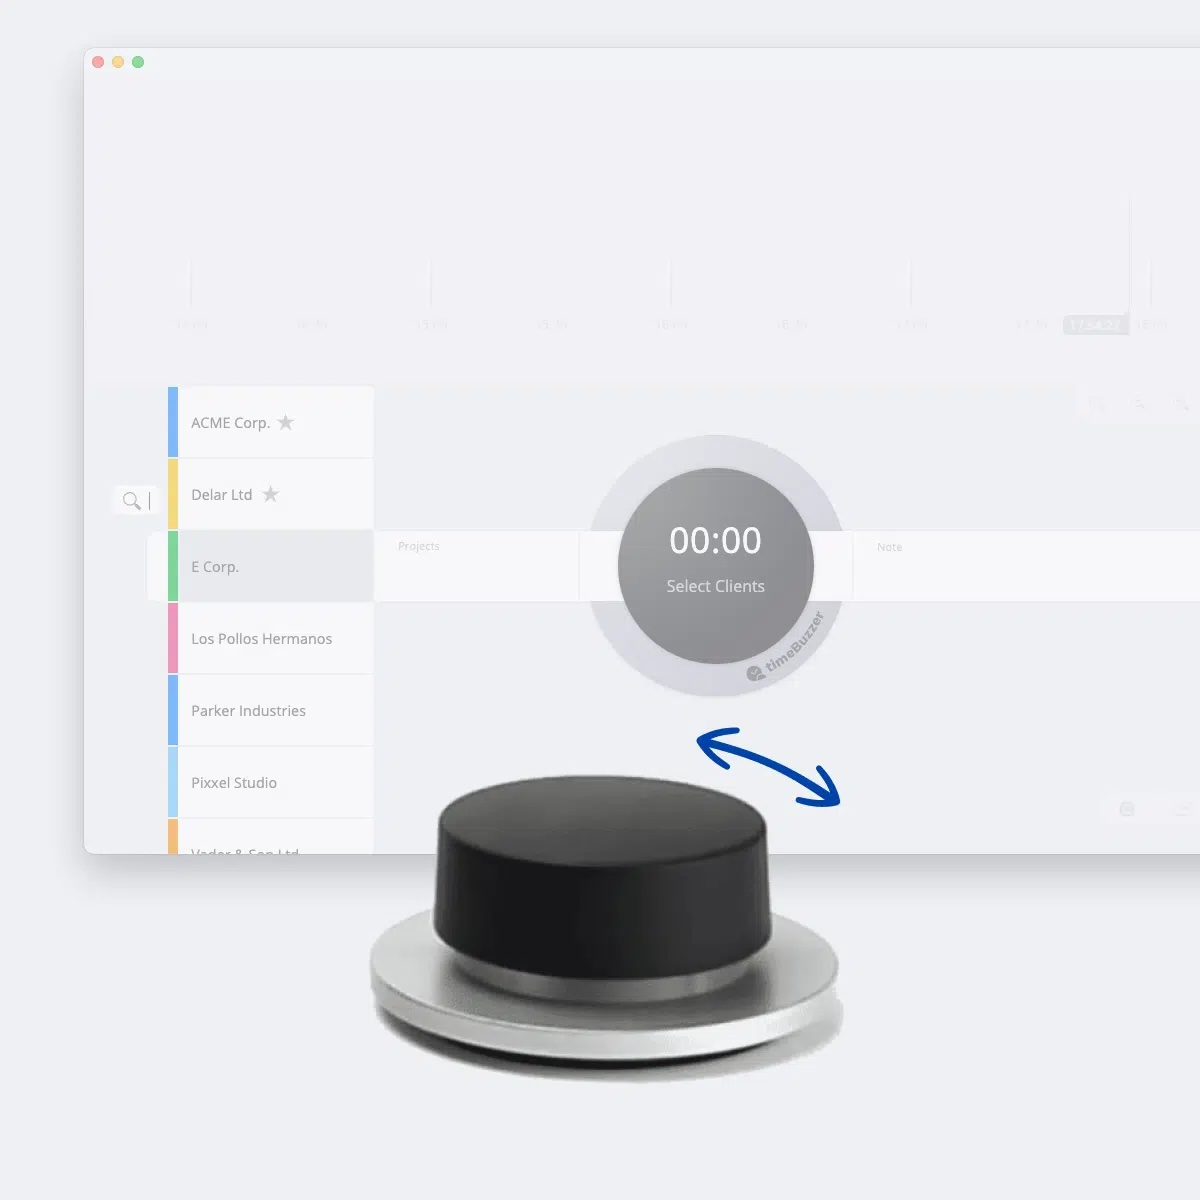
\includegraphics[width=7cm]{timebuzzer.jpeg}
		\caption{timeBuzzer – tlačítko a aplikace \cite{timebuzzer}}
		\label{pic:timebuzzer}
	\end{subfigure}
\end{figure}

Všechny ze zmíněných produktů poskytují veřejné API pro aplikace, se kterými komunikují \cite{timeflip-api} \cite{timeular-api} \cite{timebuzzer-api}. Pokud by tedy bylo potřeba produkty propojit s~vlastní aplikací, která by mohla naměřený čas spravovat, bylo by potřeba, aby aplikace komunikovala s~těmito nástroji. Pořád by byl potřeba prostředník, kterým by byla aplikace daného produktu. Výjimkou je v~těchto produktech pouze \emph{TIMEFLIP}, který poskytuje veřejný protokol pro BLE komunikaci \cite{timeflip-ble-api}. Tento produkt by tedy mohl komunikovat s~novou aplikací napřímo.

Pokud by nová aplikace měla umožňovat budoucí propojení s~jakýmkoli dalším hardwarovým produktem, tak by také měla poskytovat veřejné API, které by takovou komunikaci umožňovalo. Vývoj takových produktů by mohl být předmětem návrhu pro budoucí vylepšení aplikace.

%---------------------------------------------------------------
\subsection{Softwarové}
%---------------------------------------------------------------

Za softwarové spouštěče měření času lze považovat určité formy integrace a automatizace v~rámci zařízení, na kterém aplikace běží. V~případě aplikace na platformě iOS to mohou být následující možnosti:
\begin{itemize}
\item\textbf{Automatizace podle polohy:} Aplikace by mohla reagovat na polohu uživatele a spouštět nebo vypínat časovač na základně informace, kde se uživatel nachází. Uživatel by si mohl například nastavit určitá místa, kde by chtěl, aby se automaticky spustil časovač. Mohl by se zapnout přímo s~konkrétními přednastavenými parametry (projekt, klient, \dots), nebo by se jen mohlo ukázat upozornění, aby si uživatel časovač zapnul sám, s~parametry, které zadá. Podobně by aplikace mohla reagovat i na opuštění nějakého místa – například pokud uživatel opustí místo, které má označeno jako práci, tak by dostal upozornění, zda si nechce vypnout časovač.
\item\textbf{Automatizace podle času:} Jednoduchá forma automatizace by mohla fungovat na základě času. V~přednastavených časech by se mohl zapnout nebo vypnout časovač s~danými parametry, nebo by aplikace mohla uživatele jen upozornit.
\item\textbf{Automatizace podle kalendáře:} Užitečná by také mohla být integrace s~kalendářem uživatele. Podle naplánovaných událostí by se časovač mohl automaticky zapínat, přepínat, nebo vypínat, s~parametry z~kalendáře. Nebo opět pouze uživatele upozornit, zda si kvůli nějaké události nechce měření času aktualizovat.
\item\textbf{Automatizace podle režimu soustředění:} Systém iOS umožňuje od verze 15.0 uživatelům používat takzvané \emph{Režimy soustředění} \cite{ios-focus-modes}. Uživatel si může konfigurovat různé režimy a nastavovat, jaké mu v~tomto režimu budou chodit upozornění, jaké aplikace může používat, kdo mu může volat, apod. Od iOS verze 16 také Apple umožňuje vývojářům přizpůsobovat chování aplikace podle toho, jaký režim soustředění je zapnutý \cite{ios-focus-modes-adjustment}. Toho by se dalo vhodně využít například tak, že by se mohl automaticky spouštět časovač (nebo by uživatel mohl být upozorněn) podle toho, do jakého režimu soustředění se uživatel právě přepnul.
\item\textbf{Automatizace pomocí zkratek:} Apple nabízí uživatelům s~iOS verze 13.0 novější aplikaci \emph{Zkratky} \cite{ios-shortcuts-app}, která umožňuje tvorbu vlastních automatizujících procesů \cite{ios-shortcuts}. Tento způsob automatizace umožňuje uživatelům i~vývojářům velkou míru přizpůsobitelnosti – zkratky jdou propojovat s~dalšími aplikacemi, s~hlasovým asistentem a s~mnoha různými akcemi. Všechny předchozí způsoby automatizace jdou také nějakým způsobem vytvořit pomocí zkratek. \cite{ios-shortcuts-developer}
\end{itemize}

%---------------------------------------------------------------
\section{Existující systémy pro měření a správu odpracovaného času}
%---------------------------------------------------------------

Systémů pro měření a správu odpracovaného času existuje mnoho. Existuje dokonce několik různých článků o~tom, které systémy jsou nejlepší a jaké je jejich srovnání \cite{forbes-tracking-apps-article} \cite{zapier-tracking-apps-article}. Následující výběr příkladů je učiněn podle těchto článku, podle osobní preference a podle počtu stažení na iOS platformě.

%---------------------------------------------------------------
\subsection{Clockify}
%---------------------------------------------------------------

Clockify je jednoduchá a rozšířená aplikace primárně určená pro měření a správu odpracovaného času. Mobilní aplikace má více než 1 milion stažení \cite{clockify-app-magic} a celý systém používají miliony lidí \cite{clockify-customers}. 

V článku Forbes je hodnocena jako celkově nejlepší aplikace pro měření času pro rok 2024. Má široké spektrum funkcionalit – umožňuje měření a správu času pro různé projekty, klienty a zařízení. Mimo měření času nabízí také sledování prezence pro mzdy a účetnictví, optimalizaci produktivity zaměstnanců, měření vykazovatelného času a sdílení pokroku na projektech s~klienty. \cite{forbes-tracking-apps-article}

Clockify nabízí aplikace pro mnoho platforem: Desktopovou aplikaci pro Mac, Windows a Linux, doplněk webového prohlížeče pro Chrome, Firefox a Edge, mobilní aplikaci pro iOS a Android a nakonec sdílené Kioskové řešení, na kterém si uživatelé mohou zapisovat příchody, přestávky a další. \cite{clockify-apps}

V~základní variantě je používání aplikace zdarma. Clockify ale nabízí i~placené plány, které nabízí přidané funkce, jako audity naměřených časů, používání přestávek a další. Tyto placené plány mohou stát od \$3.99 měsíčně za uživatele až po \$11.99 měsíčně za uživatele. \cite{clockify-pricing} 

\begin{figure}[p]
	\centering
	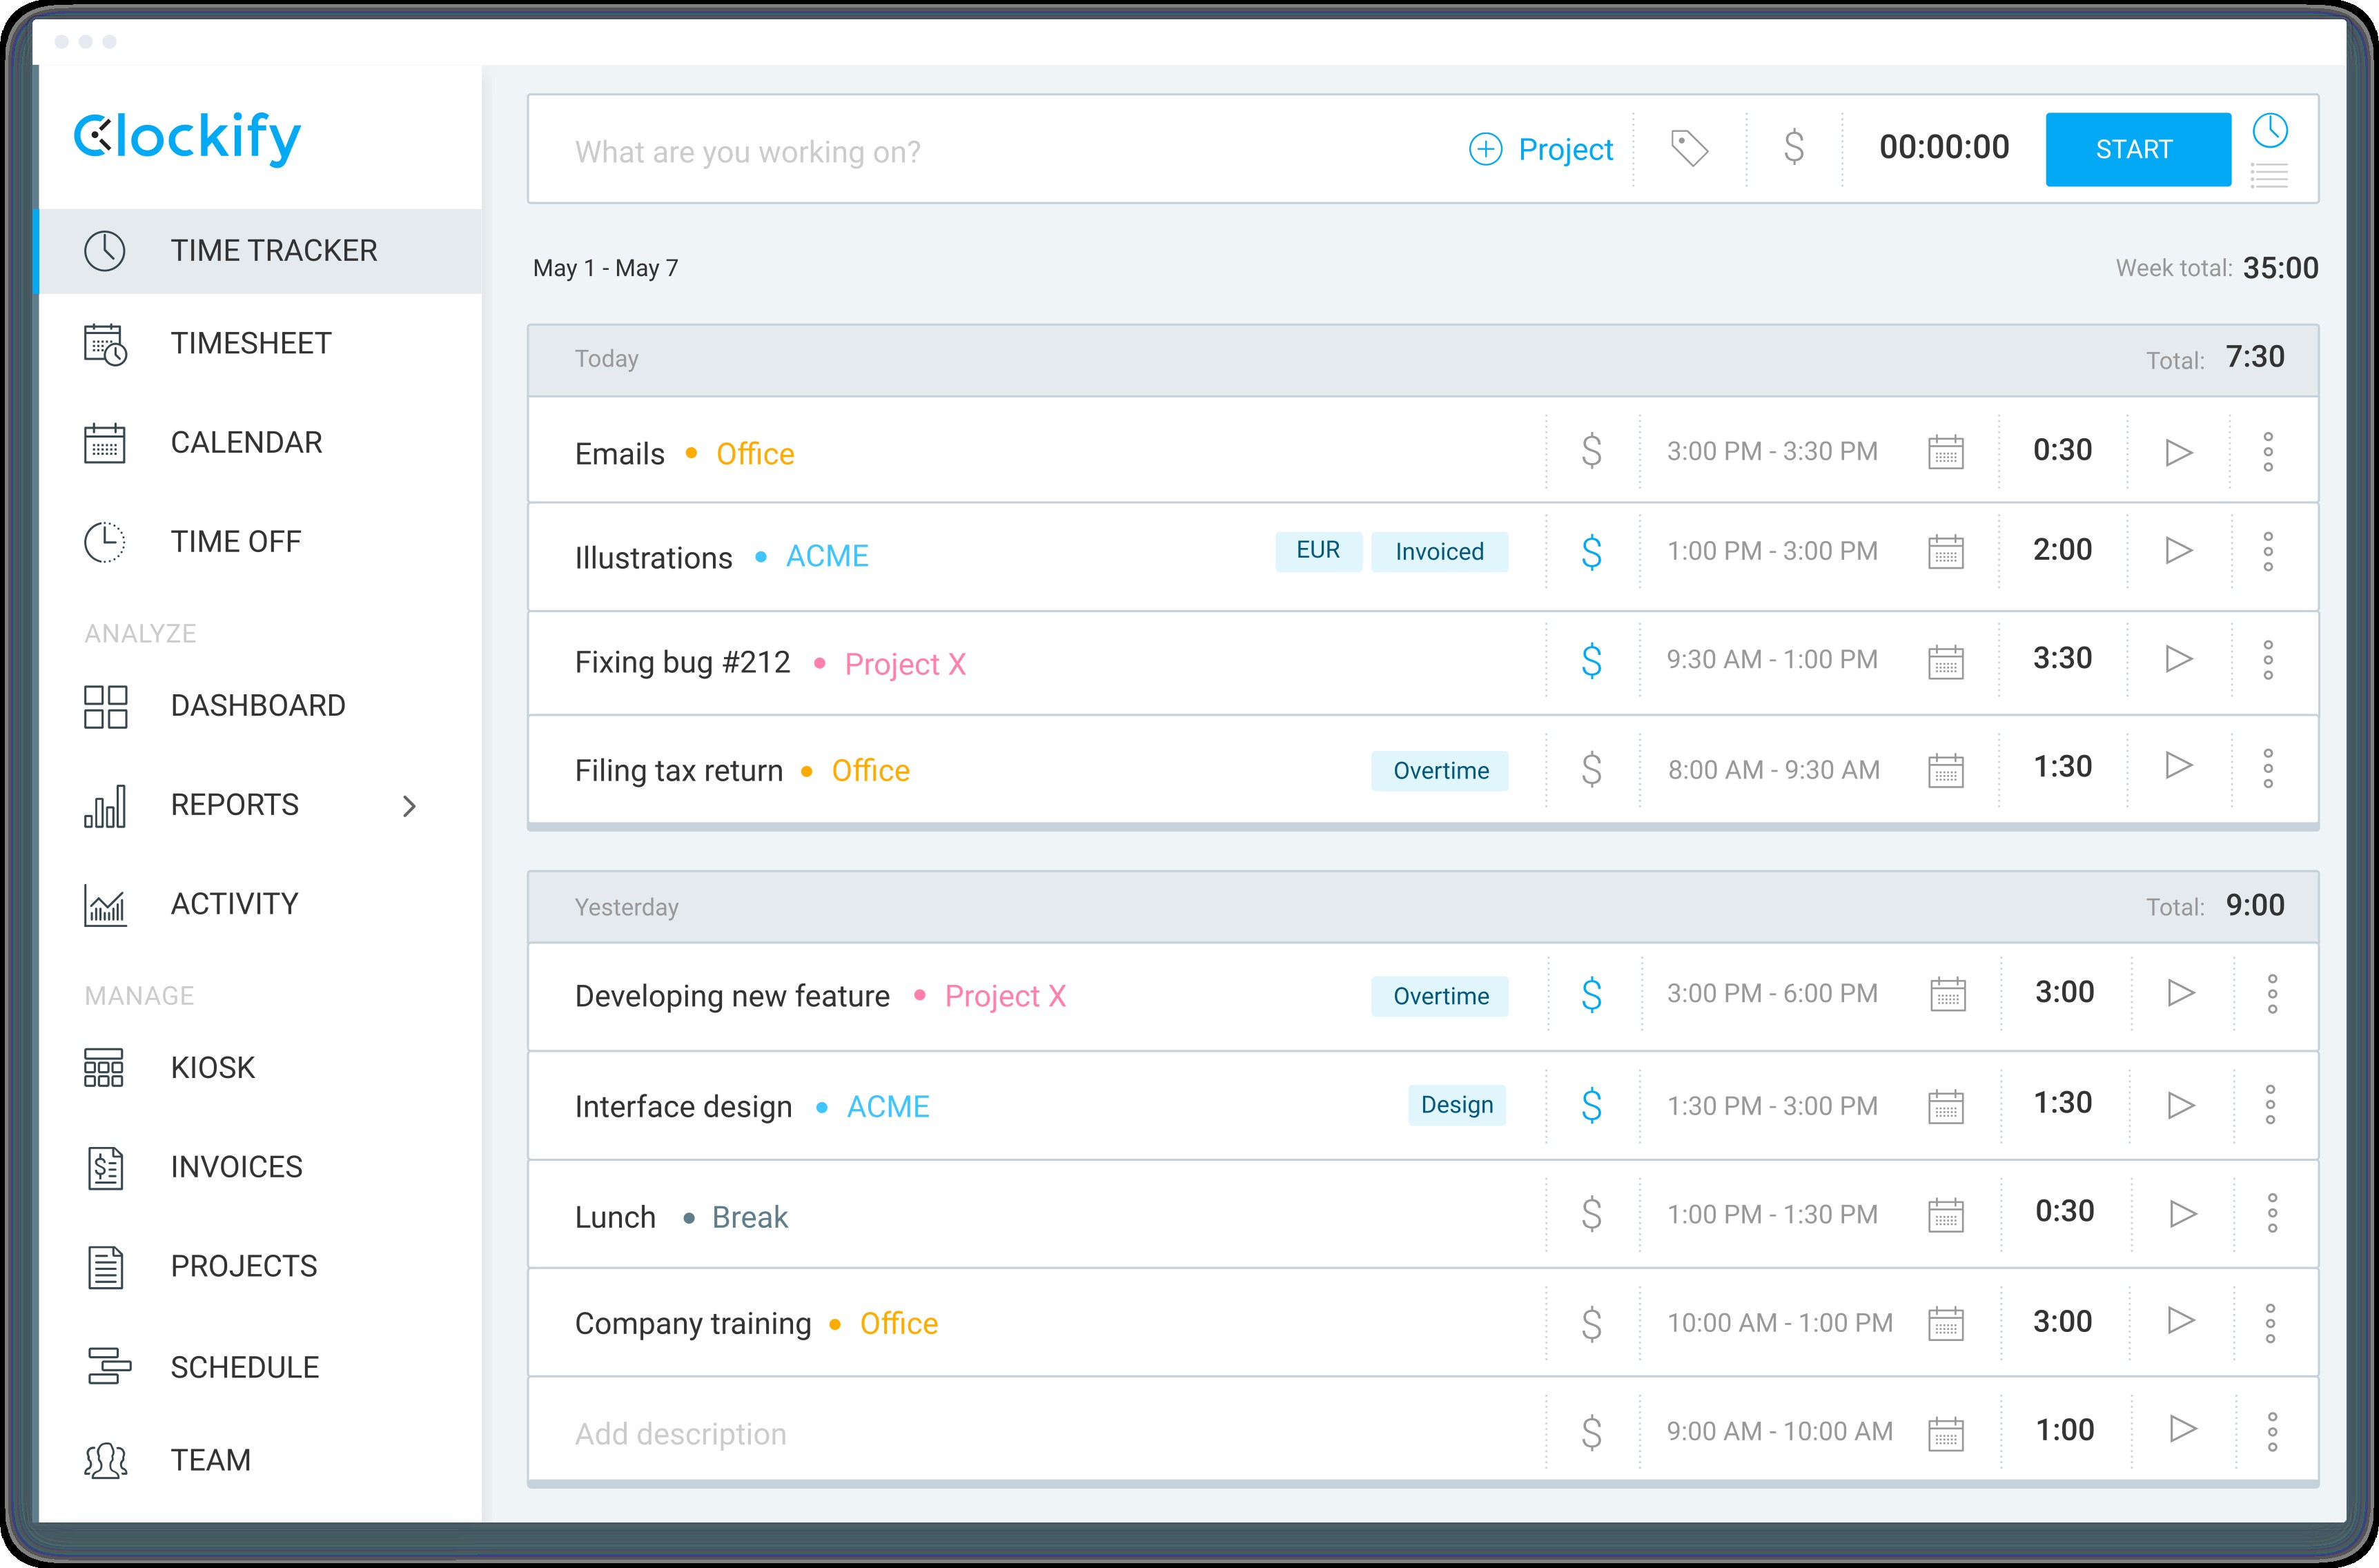
\includegraphics[width=0.9\textwidth]{clockify-timer.jpg}
	\caption{Časovač na měření času v~aplikaci Clockify \cite{clockify-features}}
	\label{fig:clockify-timer}
	\vspace{1cm}
	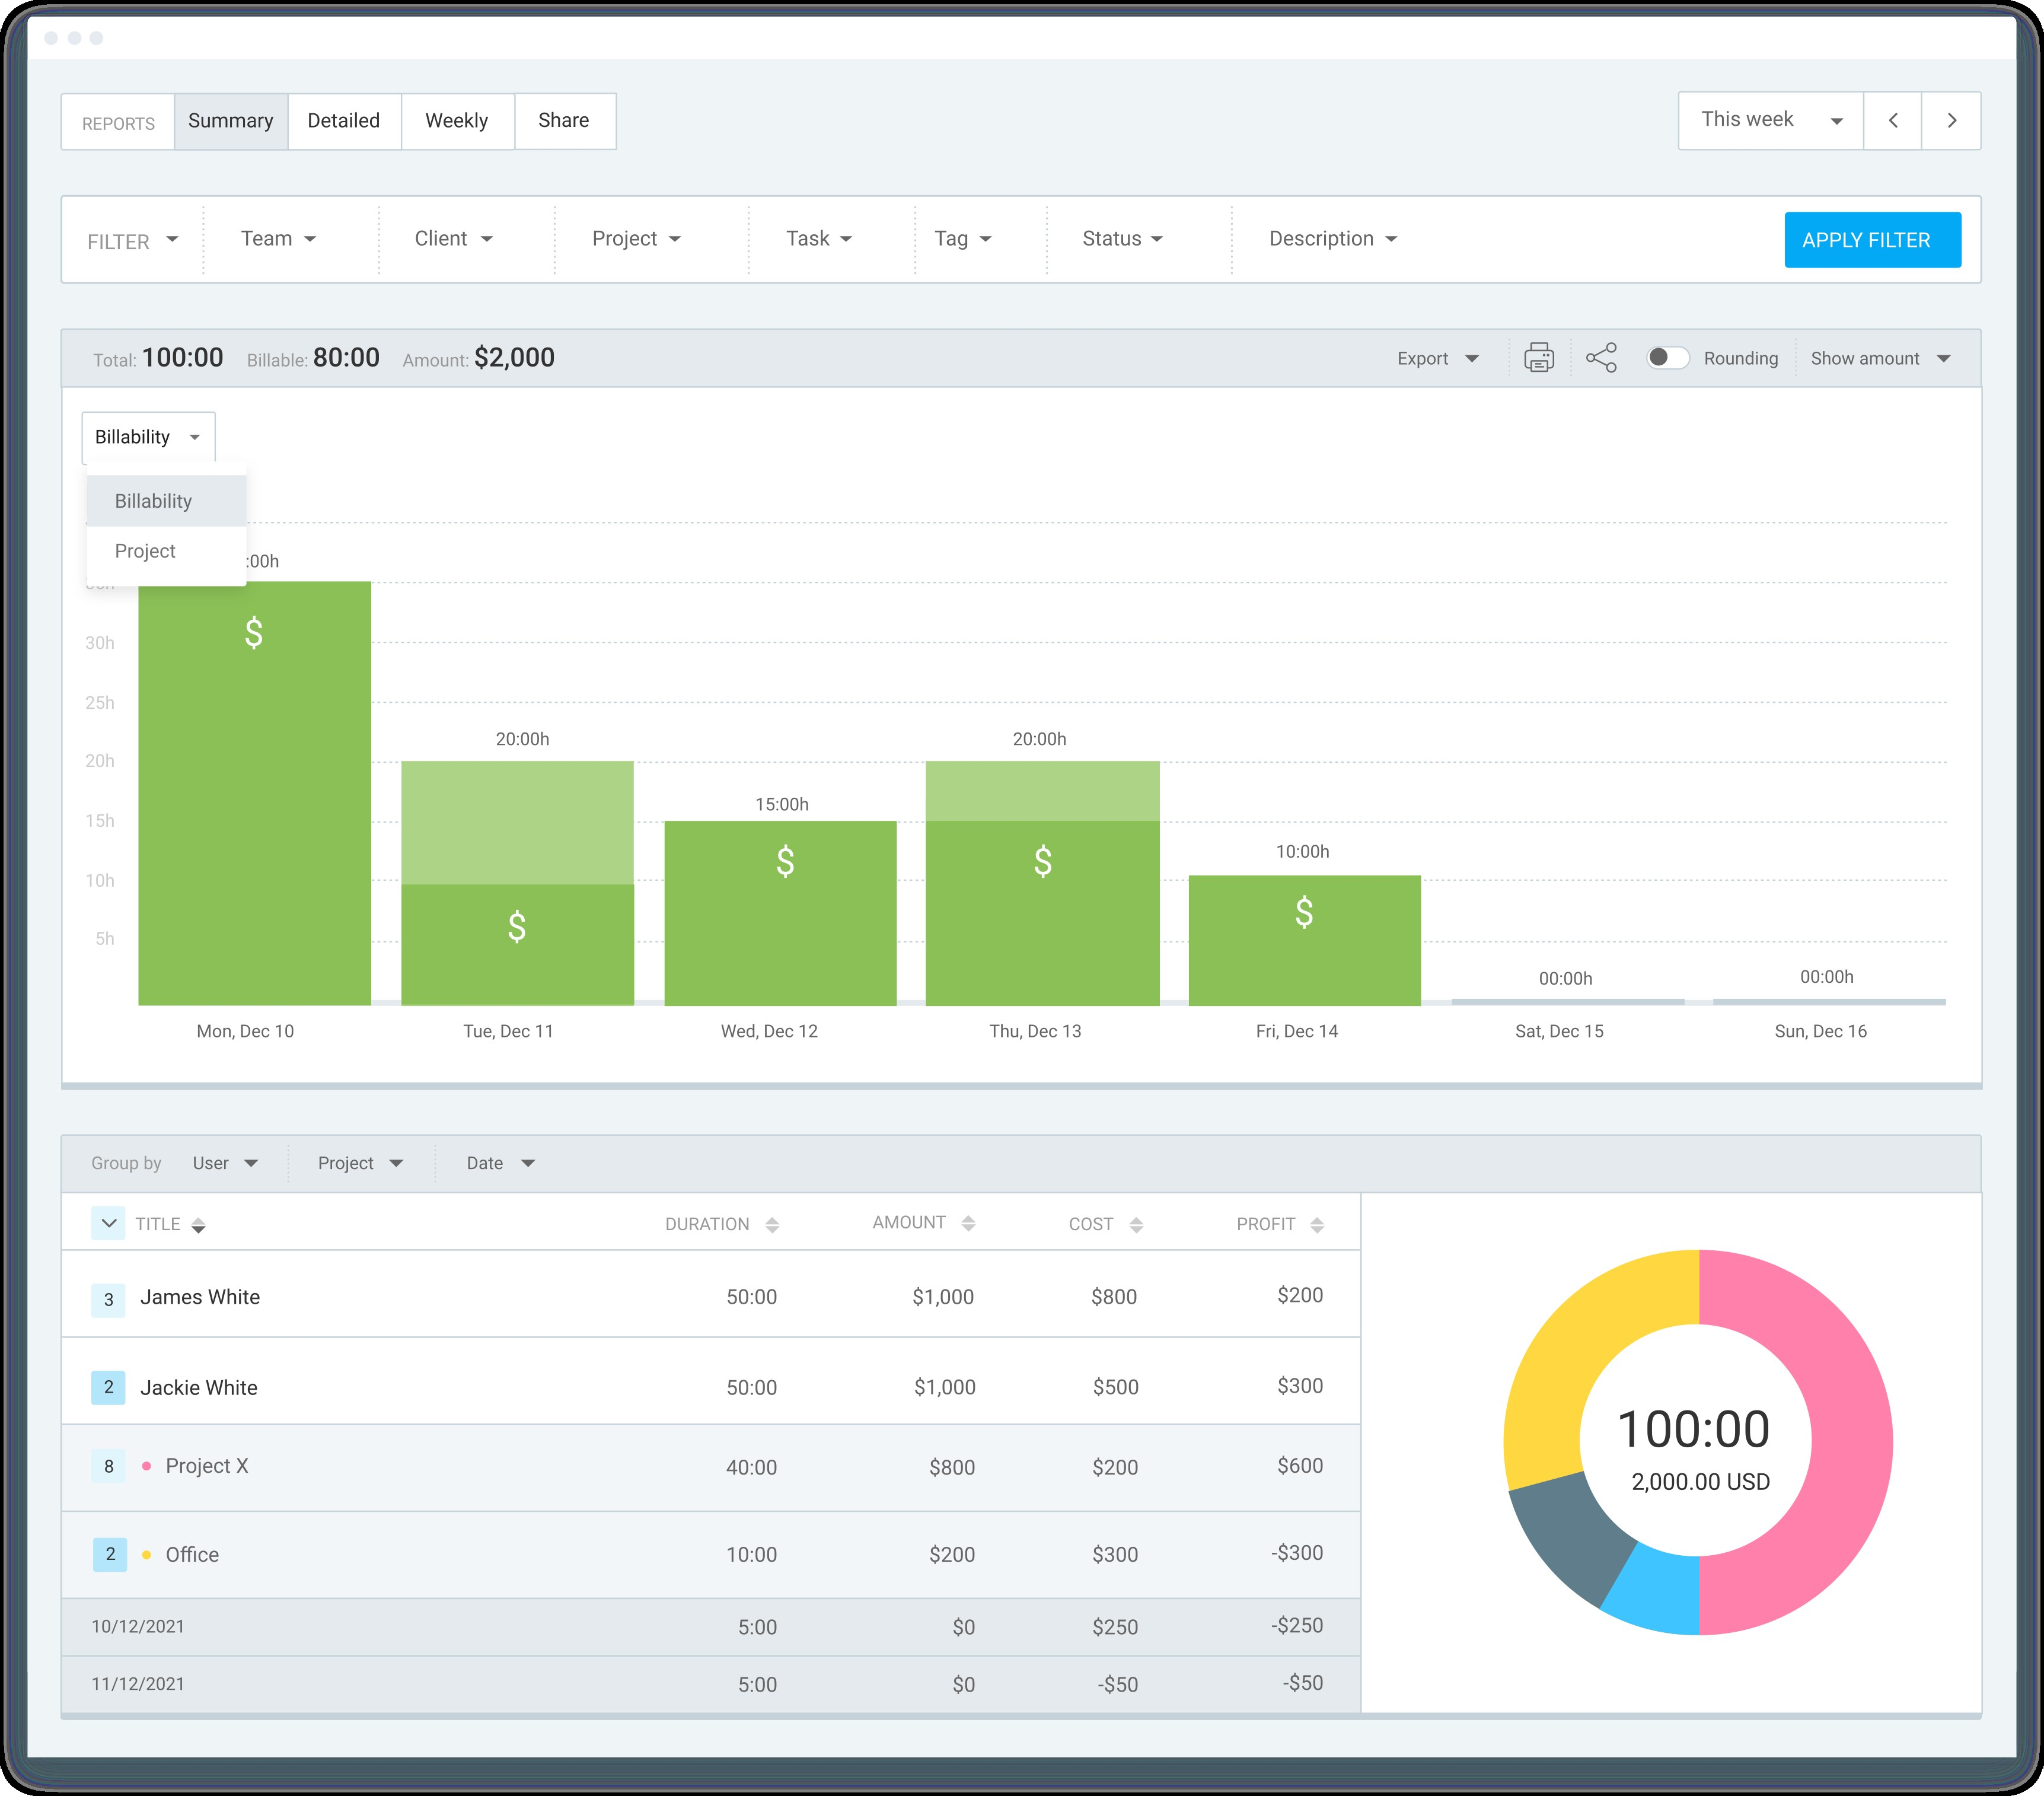
\includegraphics[width=0.9\textwidth]{clockify-report.jpg}
	\caption{Reporty v~aplikaci Clockify \cite{clockify-features}}
	\label{fig:clockify-report}
\end{figure}

Clockify nabízí dobře zdokumentované API pro své služby \cite{clockify-api}. Napojení na funkce systému lze tedy jednoduše udělat i~z~vlastního řešení. Do Clockify lze také data importovat z~CSV tabulek, jsou-li data vhodně naformátována \cite{clockify-import-timesheets}.

Mezi nevýhody systému Clockify Forbes uvádí, že projekty nejdou označit jako dokončené, a že shrnující reporty mohou být zpočátku matoucí. Celkově Clockify ale vnímá jako nejlepší řešení pro pokrytí celé škály funkcionalit.

Na obrázku \ref{fig:clockify-timer} je vidět hlavní obrazovka ve webové verzi aplikace – časovač. Uživatel si zde může časovat ručně zapnout a vypnout, přidělit projekt, přidat značky, označit vykazovatelnost a přidat popisek. Také má možnost přidat odpracovaný čas ručně, tedy ne pomocí časovače. K~tomu stačí jen napsat čas začátku a konce. Pod ovládacím panelem časovače potom uživatel vidí seznam svých již zadaných časových záznamů, které zde může jakkoli upravovat.

Dále je na obrázku \ref{fig:clockify-report} vidět obrazovka určená pro reporty. Uživatel si zde může vybrat časový úsek, pro který chce report vypracovat, a může si nastavit filtry, podle kterých chce časové vstupy filtrovat (tým, klient, projekt, úkol, značka, stav a popisek). Po aplikování filtru poté uživatel uvidí report své práce vyhovující zadaným parametrům, který si může exportovat ve formátech PDF, CSV a Excel.

%---------------------------------------------------------------
\subsection{Toggl Track}
%---------------------------------------------------------------

Toggl track je další poměrně rozšířená aplikace pro měření a správu času. Na platformě iOS má více než 1 milion stažení \cite{toggl-track-app-magic}. 

Forbes tuto aplikaci považuje za nejlepší pro malé týmy, protože nabízí plán zdarma pro týmy do 5 uživatelů a nabízí neomezený počet klientů a projektů. \cite{forbes-tracking-apps-article}

Aplikace nabízí určitou formu automatické detekce toho, že uživatel nemá zapnutý časovač, i když pracuje, nebo automatickou detekci naopak toho, že uživatel už nepracuje, ale časovač má zapnutý. Aplikace nabízí detailní denní, týdenní a měsíční reporty.

Toggl Track také pokrývá více platforem: Webovou aplikací, mobilní aplikací pro iOS a Android a desktopovou aplikací pro Windows a Mac. \cite{toggl-track}

\begin{figure}[h]
	\centering
	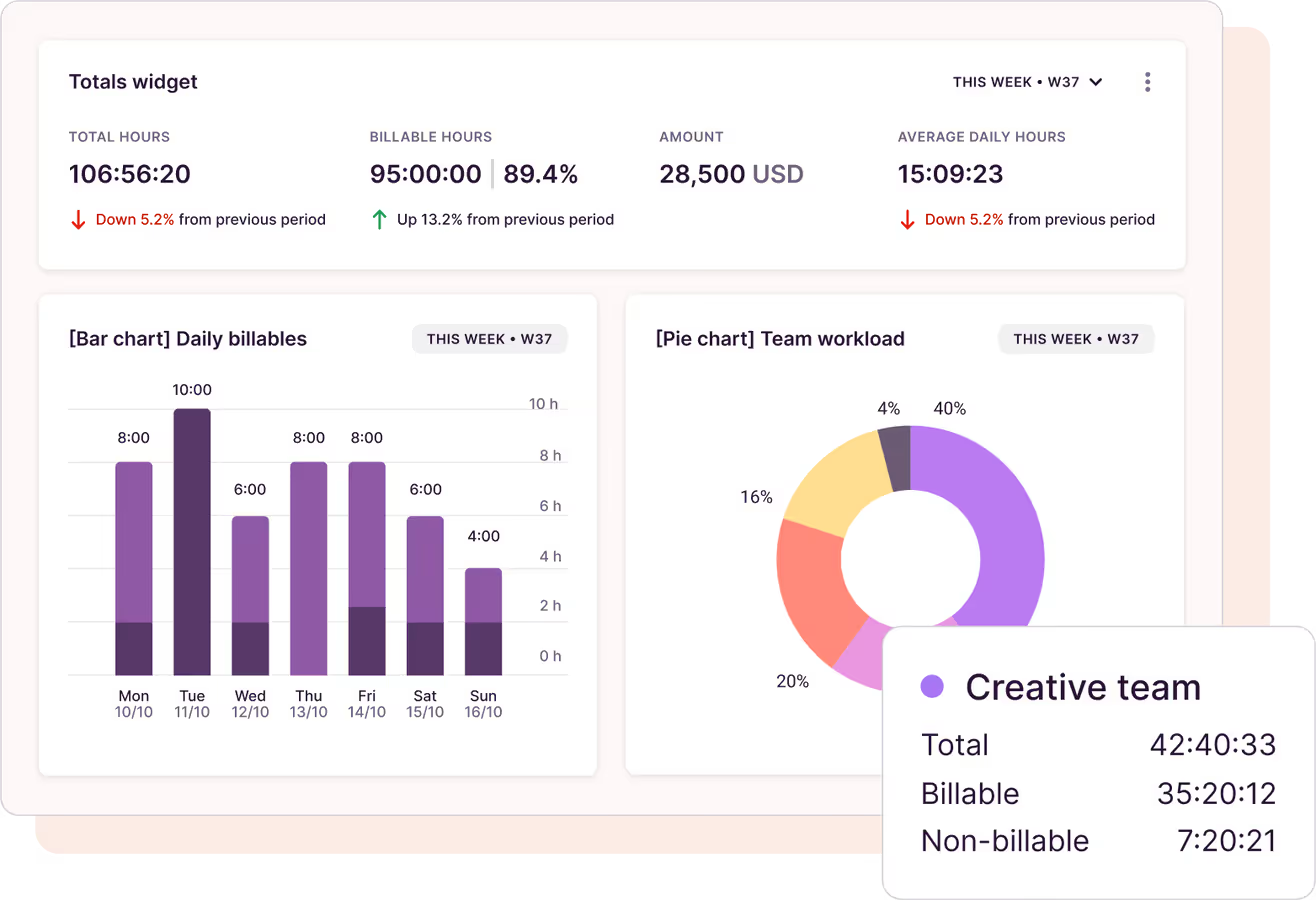
\includegraphics[width=\textwidth]{toggl-track.png}
	\caption{Aplikace Toggl Track \cite{toggl-track}}
\end{figure}

%---------------------------------------------------------------
\subsection{Deputy}
%---------------------------------------------------------------

Deputy je další aplikací, která umožňuje měření a správu odpracovaného času. Jejím hlavním účelem je však plánování směn zaměstnanců. Je uvedena jako jeden z~příkladů proto, aby šlo nahlédnout na problém měření času i~z~jiného úhlu, než striktně měření času primárně za účelem vykazování, fakturování nebo analýzy efektivity. Je také velice rozšířenou aplikací – počty stažení na mobilních telefonech překračují 5 milionů \cite{deputy-app-magic}.

Právě plánování směn zaměstnanců je hlavním důvodem, proč Forbes tuto aplikaci ve svém seznamu zmiňuje. Aplikace totiž nabízí plánování neomezeného počtu směn za měsíc. Uživatelé se mohou přihlásit k~aplikacím pro plánování a pro prezenci zvlášť. I~neplacený plán umožňuje automatické plánování směn, což šetří čas manažerům. Toto plánování umožňuje i~započítání obědových pauz, přestávek a dalšího, přímo do plánu směn, podle příslušných zákonů.  \cite{forbes-tracking-apps-article}

Deputy nabízí aplikaci pro měření odpracovaného času pro mobilní platformy iOS a Android. 

\begin{figure}[h]
	\centering
	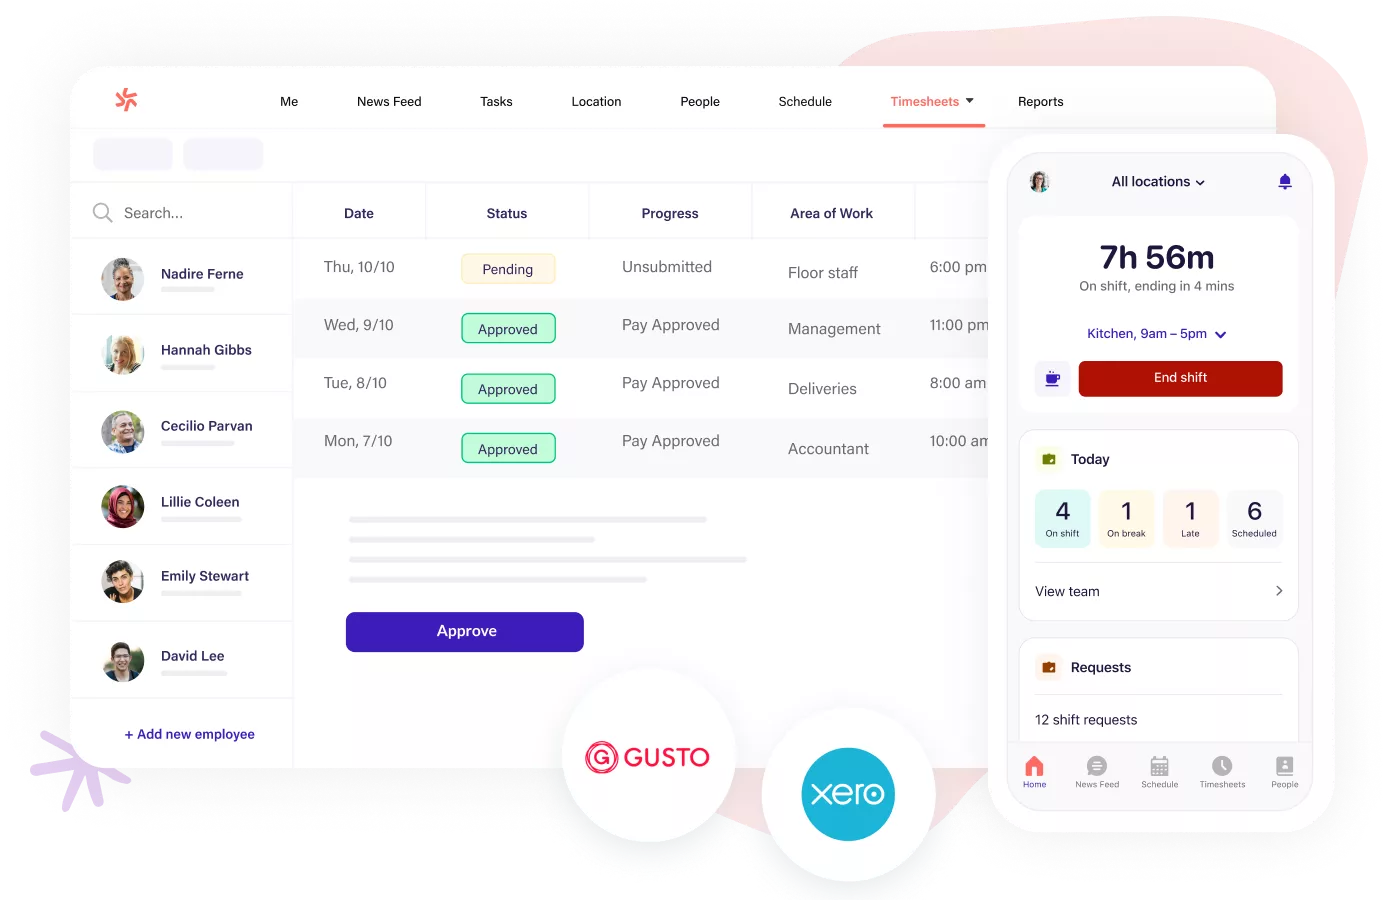
\includegraphics[width=\textwidth]{deputy.png}
	\caption{Aplikace Deputy \cite{deputy-time-tracking-app}}
\end{figure}

%---------------------------------------------------------------
\section{Vývoj mobilních aplikací pro systém iOS}
%---------------------------------------------------------------

Tato sekce se věnuje několika klíčovým tématům souvisejícím s~vývojem aplikací pro zařízení s operačním systémem iOS. Tyto témata shrnuje a poskytuje tím základ pro diskuzi o~vývoji aplikací pro tento systém.

%---------------------------------------------------------------
\subsection{Historie a vývoj iOS platformy}
%---------------------------------------------------------------

Historie operačního systému iOS začala v~roce 2007, kdy byl představen a začal se prodávat první mobilní telefon od společnosti Apple, kterým byl iPhone. V~tomto telefonu byl od výroby nainstalován operační systém, který ještě v~tu dobu nenesl název \emph{iOS}, ale \emph{iPhone OS}. Název \emph{iOS} se začal používat až později od verze systému 4. Přestože z~dnešního pohledu chybělo v~systému mnoho funkcí, se kterými si dnes mobilní telefony spojujeme, jako možnost instalace aplikací třetích stran, tak to byl v~tu dobu velký posun. Věci jako \emph{Multitouch screen}, vizuální znázornění hlasové schránky, nebo integrace s~\emph{iTunes}, byly obrovskou výhodou. Mezi předinstalované aplikace patřil kalendář, fotky, fotoaparát, poznámky, prohlížeč webu \emph{Safari}, e-mailový klient, telefon a \emph{iPod} (který se později rozdělil na aplikace pro hudbu a aplikace pro videa).

\begin{figure}[h]
	\centering
	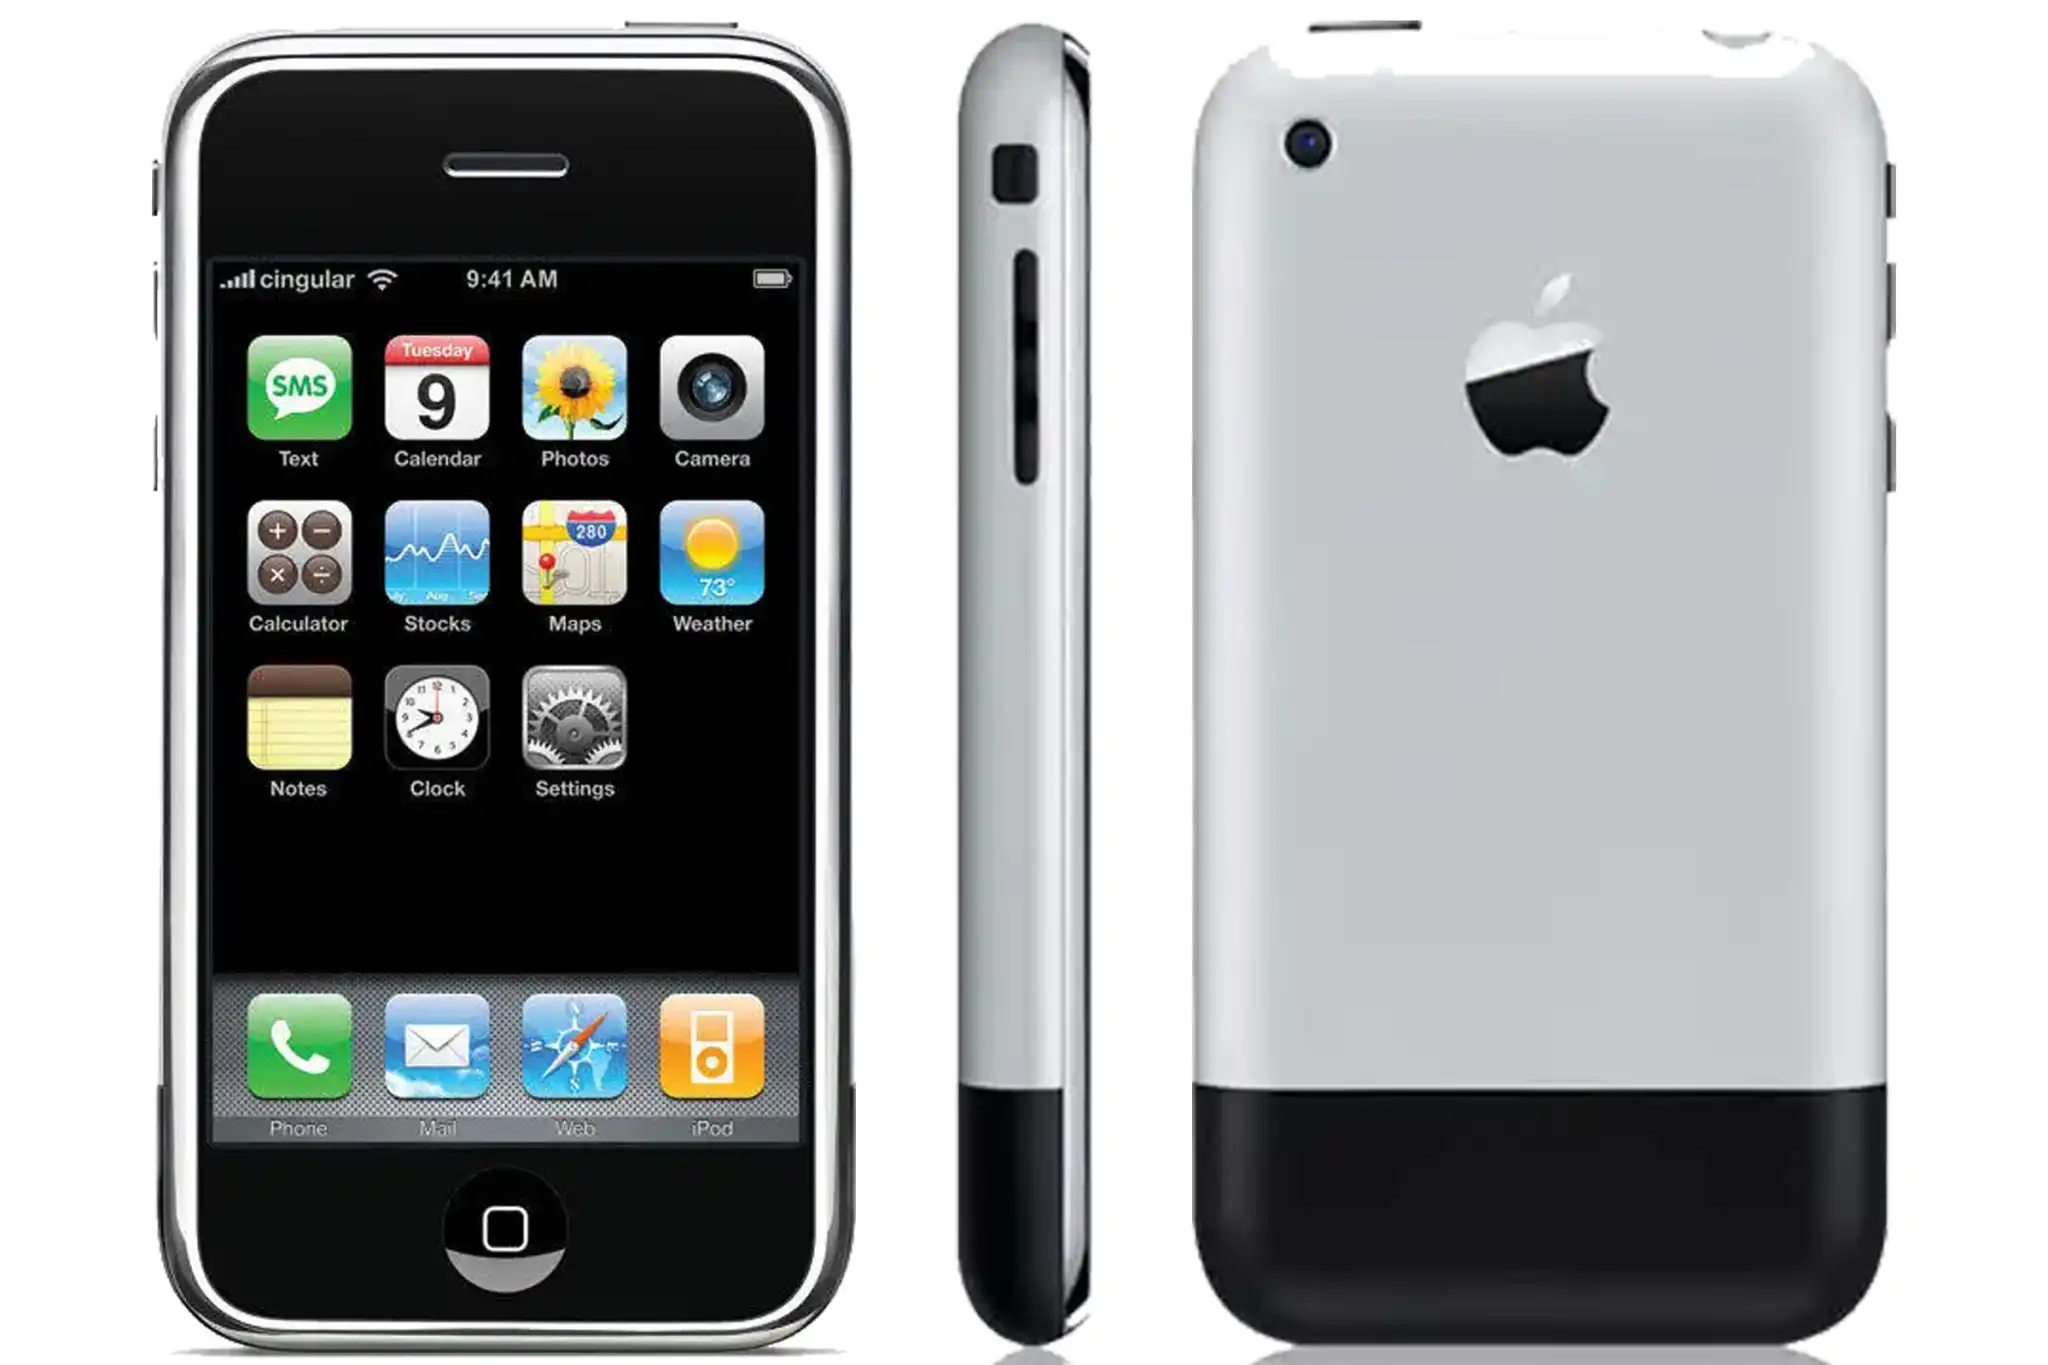
\includegraphics[width=10cm]{iphone.png}
	\caption{První model mobilního telefonu iPhone \cite{iphone-review}}
\end{figure}

O~rok později, v~roce 2008, byla představena nová generace mobilního telefonu s~názvem iPhone~3G, se kterým také vznikla nová verze operačního systému iOS (iPhone OS) 2.0. Hlavní novinkou této nové verze byl nový obchod s~aplikacemi třetích stran, \emph{App Store}. Až 500 aplikací bylo v~obchodě k~dispozici v~době, kdy byl zpřístupněn uživatelům.

V~roce 2009 poté s~novým iPhonem 3GS přišla verze iOS (iPhone OS) 3, která přinesla hlavně vylepšení, jako možnost používat kopírování a vkládání, vyhledávání přes \emph{Spotlight}, podporu MMS a možnost natáčet videa (do té doby iPhone uměl pouze pořizovat fotky). Také to byla první verze operačního systému, která fungovala i~na nových tabletech od společnosti Apple – na iPadech. První iPad byl představen v~roce 2010.

V~roce 2010 byl představen nový iPhone 4 a s~ním verze operačního systému 4. Od této verze se začal používat název \emph{iOS}, který nahradil do té doby používaný \emph{iPhone OS}. Toto nové pojmenování mělo sjednocovat názvosloví pro více zařízení – iPhone, iPad a iPod. iPhone 4 byl poměrně velkou změnou, protože disponoval novým hranatým designem a iOS 4 přineslo novinky, které tento operační systém pomalu začaly rýsovat do dnešní podoby. Mezi novinky patřil \emph{FaceTime}, \emph{multitasking}, \emph{iBooks}, organizování aplikací do složek, osobní hotspot nebo sdílení dat pomocí \emph{AirPlay} a \emph{AirPrint}. Také to byla první verze iOS, která nepodporovala všechny dosud vydané iPhony, protože nebyla kompatibilní s~prvním iPhonem.

O~rok později, s~iPhonem 4S, byl představen iOS verze 5. Apple v~ní reagoval na rostoucí trend bezdrátovosti a \emph{cloud computing} představením několika nových funkcí a platforem. Mezi ně patřil třeba iCloud nebo synchronizace s~iTunes přes Wi-Fi. Také vznikla platforma \emph{iMessage} a začalo se používat oznamovací centrum.

Dalším modelem byl iPhone 5, který poprvé změnil velikost displeje a zvětšil ji z 3,5 palce na 4. S~tímto modelem přišla verze iOS 6, kterou doprovázelo mnoho problémů. V~této verzi Apple představil hlasového asistenta \emph{Siri}, který i~přes to, že ho později předčila konkurence, byl poměrně zásadní novinkou. Dále Apple v~nové verzi představil nové aplikace pro mapy, na které do té doby používal řešení od firmy Google. Tyto mapy od začátku obsahovaly mnoho chyb a celkově byly považovány za dost nedokončené, což způsobilo ve firmě mnoho problémů.

V~roce 2013, s~novým modelem iPhone 5S, přišla verze iOS 7. Tato verze zásadním způsobem změnila vzhled uživatelského rozhraní, které se na začátku od uživatelů netěšilo příliš dobrému přijetí, ale po několika vylepšeních a po tom, co si uživatelé na nový vzhled zvykli, tak problémy ustaly. Mezi nové funkce této verze se řadí sdílení dat s~dalšími uživateli přes \emph{AirDrop}, používání operačního systému v~displejích automobilů přes \emph{CarPlay}, ovládací centrum, nebo nový způsob odemykání zařízení pomocí otisku prstu – \emph{Touch ID}.

\begin{figure}[h]
	\centering
	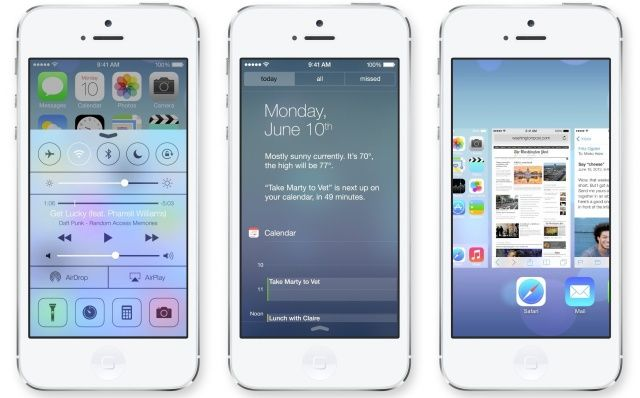
\includegraphics[width=10cm]{ios7.jpg}
	\caption{Nový vzhled iOS verze 7 \cite{ios-7-design}}
\end{figure}

S~dalším rokem a novým modelem iPhone 6 přišla verze iOS 8. iPhone 6 opět zásadně změnil svůj vzhled, ale v~operačním systému se moc zásadních změn nedělo. Apple se v~této verzi soustředil hlavně na nové funkce. Mezi ně se řadí \emph{Apple Music}, placení přes \emph{Apple Pay}, cloudové úložiště \emph{iCloud Drive}, sdílení práce mezi Apple zařízeními přes \emph{Handoff}, rodinné sdílení a další.

Rok 2015 přinesl iPhone 6S a iOS 9. V~této verzi se Apple soustředil hlavně na optimalizaci a stabilitu, příliš nových funkcí představeno nebylo – pouze nasvícení pro noční používání \emph{Night shift}, režim nízké spotřeby a možnost používat veřejný testovací beta program.

Dalším modelem byl v~roce 2016 iPhone 7 s~iOS~10. Opět nepřinesl moc nových funkcí, mimo například možnosti mazat původní nainstalované aplikace.

O~rok později poté s iPhonem~8 přišel iOS~11. V~této verzi se Apple soustředil převážně na nové funkcionality pro iPad, které se jeho použití snažily přiblížit k~plnohodnotnému počítači. Nově přibyly funkce jako podpora tužky \emph{Apple Pencil}, podpora více otevřených oken a pracovních ploch nebo prohlížeč souborů. Apple ale na závěr představení představil ještě další nový iPhone – iPhone X. Jednalo se o~další velký redesign, kdy se výrazně zvětšila plocha displeje, zmizelo přední tlačítko a vzniklo ověření uživatele pomocí obličeje – \emph{Face ID}.

V~roce 2018 Apple představil iPhone~XS a levnější variantu XR, se kterými přišel iOS~12, kde se jednalo opět jen o~mírná vylepšení. 

S~dalším rokem přišel iPhone~11 a iOS~13. Tento systém už se rozdělil – pro zařízení iPad nyní vznikl oddělený \emph{iPadOS}. V~iOS~13 Apple představil možnost tmavého režimu pro celý systém, nové možnosti bezpečnosti a soukromí a s~tím související možnost přihlášení přes Apple.

V~roce 2020 s~iPhonem~12 a iOS~14 Apple přidal několik menších změn a vylepšení, jako \emph{Widgety} na domovské obrazovce.

Podobně to bylo i~v~roce 2021, kdy Apple s~novým iPhonem~13 a iOS~15 přidával velké množství menších vylepšení, primárně do vlastních aplikací.

S~rokem 2022 přišel iPhone~14 a iOS~16, který přinesl sadu vylepšení a nových funkcí pro zamčenou obrazovku, spolu s~dalšími vylepšeními,

Poslední velký update iOS přišel v~roce 2023 s~iPhonem~15 a iOS~17. A jak už bylo v~posledních letech zvykem, tak tato aktualizace přinášela větší množství menších vylepšení a aktualizací, které ale už nijak zásadně neměnily systém a interakci s~ním. \cite{history-of-ios}

Za těchto 17 let vývoje se operační systém iOS dostal do stavu, kdy ho v~současnou chvíli používá $1,46$ miliard aktivních uživatelů. Mobilních telefonů iPhone se od roku 2007 prodalo $2,3$ miliard. \cite{iphone-user-statistics}

%---------------------------------------------------------------
\subsection{Vývojové nástroje a prostředí}
%---------------------------------------------------------------

Jak již bylo zmíněno v~předchozí sekci, obchod s~aplikacemi \emph{App Store} byl uživatelům dostupný od roku 2008. Ve stejnou dobu také Apple zpřístupnil vývojářům iPhone SDK ve svém vývojovém prostředí \emph{Xcode}. Toto vývojové prostředí od Applu již existovalo od roku 2003, kdy vzniklo jako rebranding původního vývojového prostředí \emph{Project Builder}. S~příchodem App Storu Apple umožnil všem vývojářům v~Xcodu vyvíjet aplikace pro iPhone OS od verze 2.0 pomocí zmíněného iPhone SDK. 

Vývojové prostředí Xcode je jednotné integrované vývojové prostředí, které slouží pro vývoj aplikací pro všechny platformy společnosti Apple. Lze stáhnout zdarma z~obchodu \emph{Mac App Store} nebo ze stránek společnosti Apple. Instalace vývojového prostředí obsahuje i~instalaci dalších pomocných nástrojů, jako je simulátor zařízení (iPhone, iPad, \dots), nástroje příkazové řádky, a další. \cite{xcode-history}

Pro nativní vývoj iOS aplikací se dříve používal programovací jazyk \emph{Objective-C} \cite{objc} a pro tvorbu uživatelského rozhraní knihovna \emph{UIKit}. V~roce 2014 Apple přidal podporu svého nového programovacího jazyku \emph{Swift} \cite{swift} a v~roce 2019 přidal podporu nové deklarativní knihovny pro tvorbu uživatelského rozhraní \emph{SwiftUI} \cite{swiftui}.

%---------------------------------------------------------------
\subsection{Architektura aplikací}
%---------------------------------------------------------------

Jako u~každého softwarového projektu, architektura je důležitou součástí jeho návrhu. K~architekturám mobilních aplikací existuje mnoho přístupů. Například u~Android aplikací sám Google doporučuje, jaké architektonické vzory by měly být používány a doporučuje architektury pro tyto aplikace \cite{android-app-arch}. Apple přímo žádné architektury pro aplikace cílící na iOS platformu nedoporučuje. 

Dokumentace pro iOS platformu ale obsahuje mnoho ukázek kódu věnujících se konkrétním tématům (například \cite{swift-ui-tutorial-complex-interfaces}), kde je vždy nějaký náznak architektury připraven. V~těchto ukázkách se vyskytuje architektura \emph{Model-View-Controller} (zkráceně MVC). Narozdíl od tradiční MVC architektury se ta používaná Applem mírně liší, jelikož tradiční MVC architektura není moc dobře aplikovatelná na moderní iOS vývoj. Jak lze vidět na obrázcích \ref{fig:mvc}, v~tradičním MVC by mělo \emph{View} být beze stavu a měl by ho pouze překreslovat \emph{View Controller}. Toto sice je možné v~iOS aplikaci implementovat, ale nedává to moc smysl, protože všechny tyto 3 entity jsou hluboce provázané, což dramaticky snižuje jejich opětovné použití. Při použití v~iOS aplikaci je \emph{Controller} mediátorem mezi \emph{View} a \emph{Model}, kteří o~sobě navzájem nic nevědí. Jelikož je ale \emph{View Controller} zpravidla velice provázán s~\emph{View}, tak vzniká potřeba psát masivní \emph{View Controller}. Proto se v~iOS vývoji často referuje na MVC jako na \emph{Massive View Controller}.

\begin{figure}[h]
	\centering
	\begin{subfigure}[b]{0.35\textwidth}
		\centering
		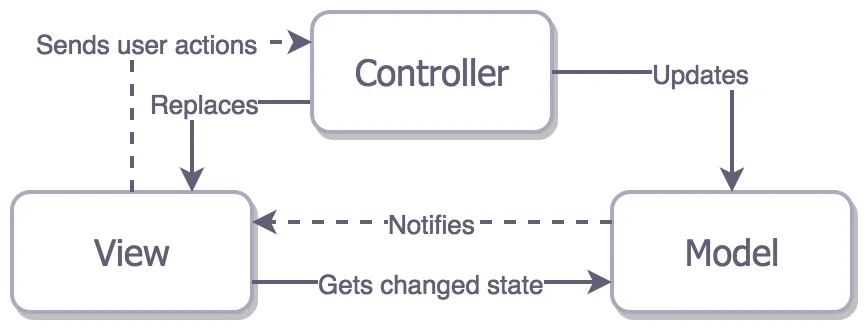
\includegraphics[width=6cm]{traditional-mvc.png}
		\caption{Tradiční MVC architektura}
	\end{subfigure}
	\hspace{1cm}
	\begin{subfigure}[b]{0.45\textwidth}
		\centering
		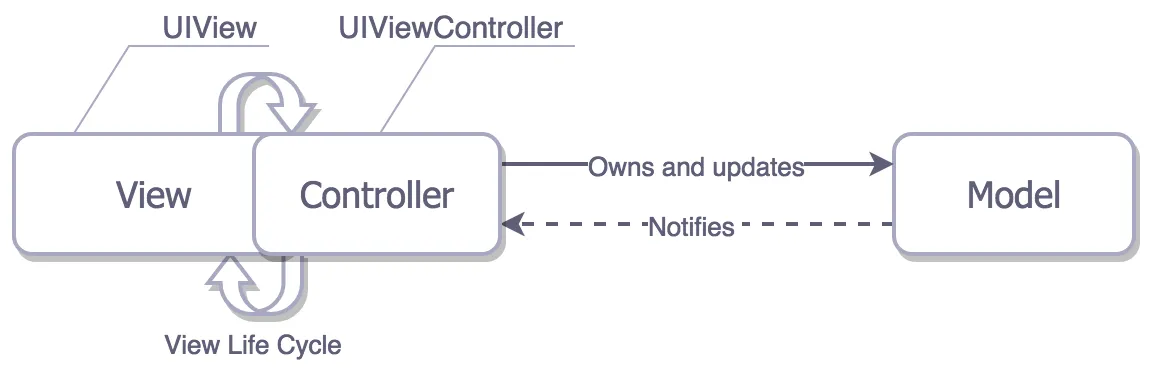
\includegraphics[width=7cm]{apple-mvc.png}
		\caption{MVC architektura v~iOS aplikacích}
	\end{subfigure}
	\caption{Architektura Model-View-Controller \cite{ios-architecture-patterns}}
	\label{fig:mvc}
\end{figure}

Architektura MVC je ale v~ukázkách kódu od Applu používána pravděpodobně převážně proto, protože se hodí pro výstižné a krátké ukázky kódu – obsahuje totiž minimální \emph{overhead}. Pro potřeby větších projektů začíná být nedostačující. Nelze nijak testovat logika prezentování, a \emph{View} také nelze pomocí jednotkových testů otestovat. Jediné, co lze testovat, je \emph{Model}. A velkou nevýhodou je právě zmíněný masivní \emph{View Controller}, který pro složitější obrazovky přestává být přehledný.

Velmi rozšířenou architekturou v~iOS vývoji je \emph{Model-View-ViewModel} (zkráceně MVVM). \emph{View} a \emph{Model} zastávají stejnou funkci jako v~MVC, a mediátorem je zde \emph{View Model}. \emph{View} je v~tomto případě konkrétní obrazovka a/nebo \emph{View Controller}. \emph{View Model} je nezávislý na knihovně uživatelského rozhraní, což umožňuje jeho lepší testovatelnost. Drží stav obrazovky, vyvolává změny pro \emph{Model} a aktualizuje se podle něj. Vizuální reprezentace architektury MVVM lze nahlédnout v~obrázku \ref{fig:mvvm}.

\begin{figure}[h]
	\centering
	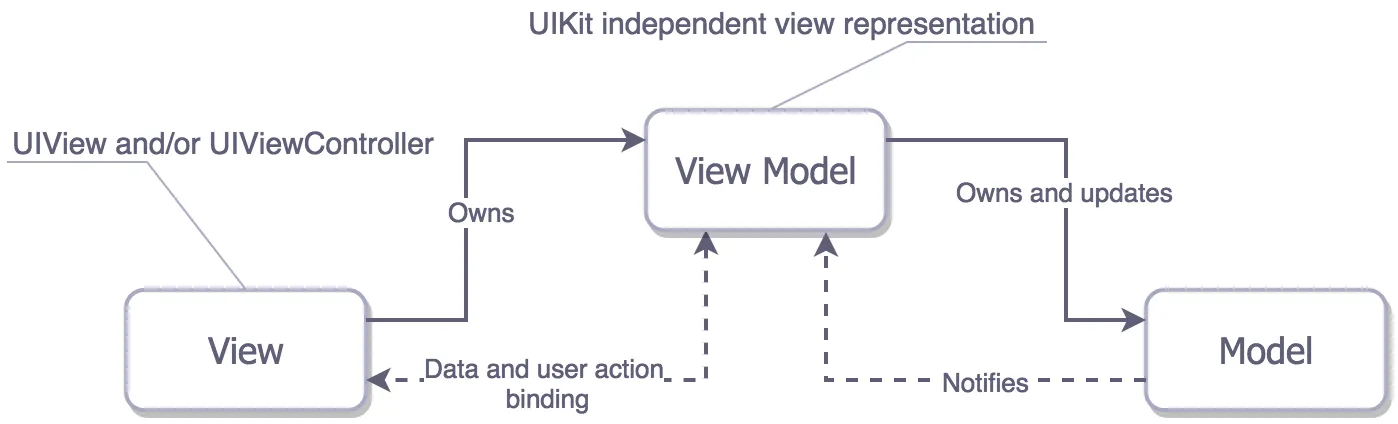
\includegraphics[width=10cm]{mvvm.png}
	\caption{Architektura MVVM \cite{ios-architecture-patterns}}
	\label{fig:mvvm}
\end{figure}

Další rozšířenou architekturou v~iOS aplikacích je \emph{Viper}. Tato architektura nepochází ze skupiny MV(X). \emph{Viper} se snaží vzít rozdělovaní odpovědností o~krok dále – obsahuje 5 vrstev:
\begin{itemize}
\item\textbf{View:} Zastává stejnou funkcionalitu jako v MV(X), tedy \emph{View} a/nebo \emph{View Controller}.
\item\textbf{Interactor:} Obsahuje byznysovou logiku související s~daty, jako tvorba instancí nebo načítání dat ze serveru.
\item\textbf{Presenter:} Obsahuje byznysovou logiku UI, ale je nezávislý na UI knihovně. Volá metody \emph{Interactoru}.
\item\textbf{Entities:} Čisté objekty dat.
\item\textbf{Router:} Odpovědný za přechody mezi \emph{Viper} moduly.
\end{itemize}
Tato architektura je poměrně volná v~tom, co bude konkrétní \emph{Viper} modul reprezentovat. Může to být jedna samotná obrazovka, ale může to být celá část aplikace. Lze si všimnout několika rozdílů od architektur ze skupiny MV(X):
\begin{itemize}
\item Model (interakce s~daty) je přesunut do \emph{Interactoru} pomocí \emph{Entities}.
\item Pouze povinnosti UI reprezentace \emph{Controlleru}/\emph{View Modelu} je přesunuta do \emph{Presenteru}, ale ne byznysová logika s~daty.
\item \emph{Viper} explicitně adresuje odpovědnost navigace, kterou řeší \emph{Router}.
\end{itemize}
Vizualizace architektury \emph{Viper} lze nahlédnout v~obrázku \ref{fig:viper}. \cite{ios-architecture-patterns}

\begin{figure}[h]
	\centering
	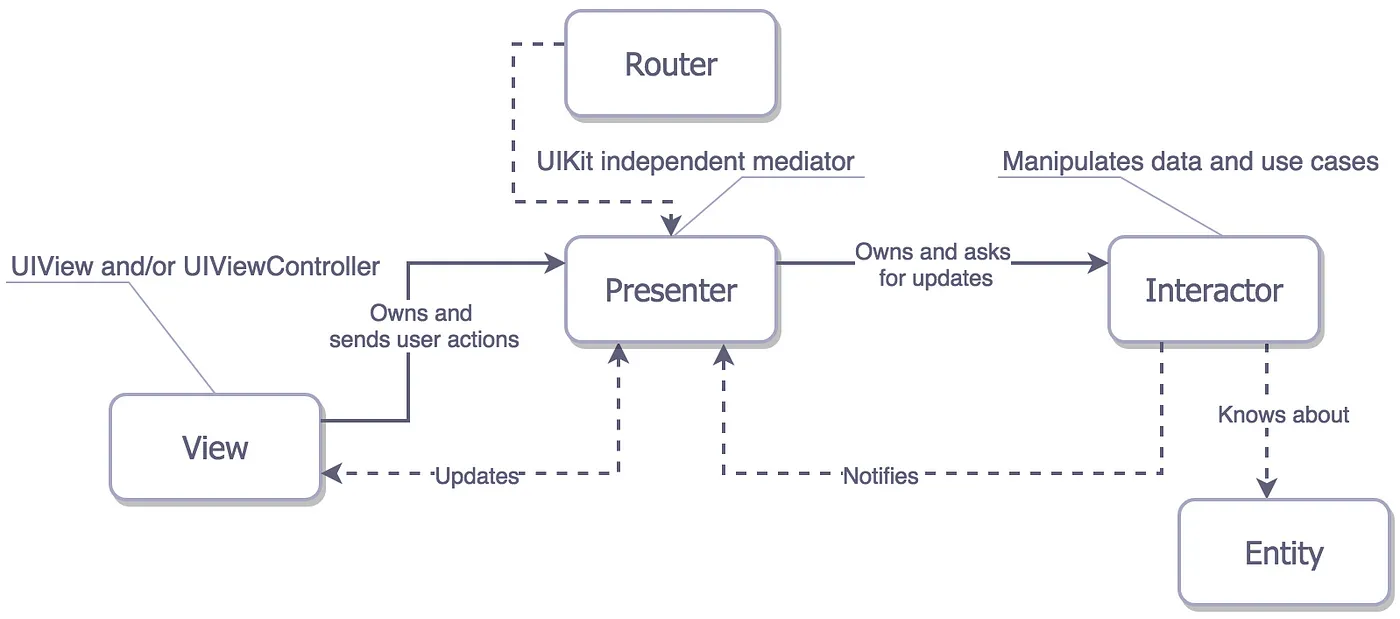
\includegraphics[width=12cm]{viper.png}
	\caption{Architektura \emph{Viper} \cite{ios-architecture-patterns}}
	\label{fig:viper}
\end{figure}

Existuje také rozšíření architektury MVVM o~navigační logiku, takzvaná MVVM-C, kde písmeno C představuje \emph{Flow Coordinator}. Tato vrstva je odpovědná za navigační tok, vytváří instance \emph{View} a/nebo \emph{View Controller} a prezentuje je, předává data mezi těmito instancemi a obsluhuje akce uživatele. Struktura \emph{Flow Coordinatoru} je vhodně navržena tak, aby se dala také dobře testovat. \cite{ios-mvvm-c}

Jednotlivé architektury mají také své aktualizované varianty pro nově používanou deklarativní UI knihovnu \emph{SwiftUI}. Všechny ze zmíněných architektur se dají vhodně použít i~s~touto knihovnou. Ve \emph{SwiftUI} už se jednotlivé obrazovky nerozdělují na \emph{View} a \emph{View Controller}, ale zůstává zde pouze \emph{View}. \emph{SwiftUI} ale ze své podstaty jako deklarativní knihovna přináší nové možnosti, jak k~architektuře aplikace přistupovat.

Jednou z~novějších architektur, které využívají výhody deklarativních UI knihoven, jako je \emph{SwiftUI}, je \emph{Model-View-Intent} (zkráceně MVI). \emph{View} a \emph{Model} reprezentují stejné vrstvy jako doposud a \emph{Intent} reprezentuje nějaký úmysl vyvolat určitou akci. Tím může být například kliknutí uživatele. Konkrétní \emph{Intent} poté pomocí nějaké byznysové logiky aktualizuje stav, podle kterého se následně aktualizuje \emph{View}. \cite{swiftui-mvi}





















